\documentclass[12pt]{article}
\usepackage[utf8]{inputenc}
\usepackage{amsmath}
\usepackage{mathtools}
\usepackage{amsfonts}
\usepackage{lastpage}
\usepackage{tikz}
\usepackage{pdfpages}
\usepackage{gauss}
\usepackage{fancyvrb}
\usepackage{fancyhdr}
\usepackage{graphicx}
\pagestyle{fancy}
\fancyfoot[C]{\footnotesize Page \thepage\ of 5}
\DeclareGraphicsExtensions{.pdf,.png,.jpg}
\title{Lynopgave 1}
\author{Nikolaj Dybdahl Rathcke and Victor Petren Bach Hansen}
\chead{Nikolaj Dybdahl Rathcke (rfq695) - Victor Petren Bach Hansen (grn762)}

\begin{document}
\section*{MatIntroNat - Lynopgave 1}
\subsection*{1.1}
Betragt funktionerne $f_1$ og $f_2$ 	givet ved
$$f_1(x)=\frac{x^2-7}{x+\sqrt{7}}\:\:og\:\:f_2(x)=\frac{x^2-7}{x+2.645751311}$$
Lav et Maple-plot af graferne for de to funktioner med $x$ i intervallet [-2.6458, -2.6457]. Forklar, hvad du ser.\\
\begin{center}
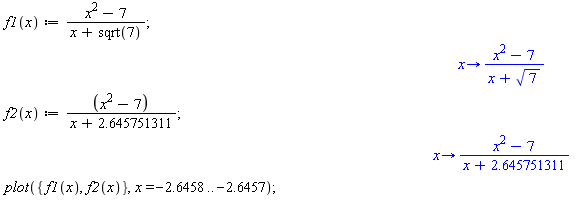
\includegraphics[scale=0.6]{1.png}
\end{center}
\begin{center}
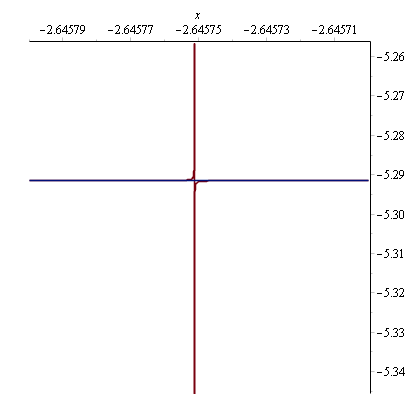
\includegraphics[scale=0.6]{2.png}
\end{center}
Der ses ud fra figuren, at det er en dårlig afrunding af kvadratrodden i nævneren, da funktionerne ellers ville have ligget oven i hinanden. Netop til x-værdien $-2.645751311$ vil $f_2$ prøve at dividere med 0, hvilket ikke er muligt. Da $\sqrt{7}$ er irrationel og ikke har en eksakt værdi (da det er en uendelig talrække) vil der i $f_1$ aldrig deles med nul, mens den dog vil prøve, og fejle, for $f_2$, hvilket resulterer i hoppet i grafen.
\subsection*{1.2}
\subsubsection*{a}
Lad $z=3+4i$ og $w=2+i$, beregn følgende:
$$z-2w, z+w, z * w, \dfrac{z}{w}, w^2$$
Til at udregne disse resultater er der blevet benyttet regnereglerne på side 111 i Kalkulus (3.1.4)\\
$z-2w= (3+4i)-2(2+i)=(3+4i)-(4+2i)=(3-4)-i(4-2)=-1-2i$\\ \\
$z+w=(3+i)i+(2+i)=(3i+4i^2)+(2+i)=(3i-4)+(2+i)=4i-2$\\ \\
$z * w=(3*2-4*1)+i(3*1+4*2)=2+11i$\\ \\
$\dfrac{z}{w}=\dfrac{3+4i}{2+i}=\dfrac{3*2+4*1}{2^2+1^2}+i\dfrac{4*2-3*1}{2^2+1^2}=2+i$\\ \\
$w^2=(2*2-1*1)+i(2*1+2*1)=3+4i$

\subsubsection*{b}
Find modulus og argument for $w$\\
\\
Modulus er lig med længden af vektoren, som fås ved formlen: $\sqrt{a^2+b^2}$ hvor $a$ og $b$ læses ud fra de komplekse tal der er på formen: $z=a+bi$\\
Modulus, eller $r$, er derfor:
$$r=\sqrt{2^2+1^2}=\sqrt{5}$$
Herefter findes argumentet til at være:
$$cos\phi=\dfrac{2}{\sqrt{5}}, sin\phi=\dfrac{1}{\sqrt{5}}$$
Altså er det:\\
$$ \arctan(\dfrac{1}{2})$$
\subsection*{1.3}
\subsubsection*{a}
Udregn modulus og argument af det komplekse tal:
$$\frac{(\frac{3}{4}+\frac{1}{2}i)(\frac{1}{4}-\frac{3}{2}i)}{(-\frac{1}{4}+\frac{1}{2}i)i}$$
Ved hjælp af Maple, kan vi udregne disse værdier således:
\begin{center}
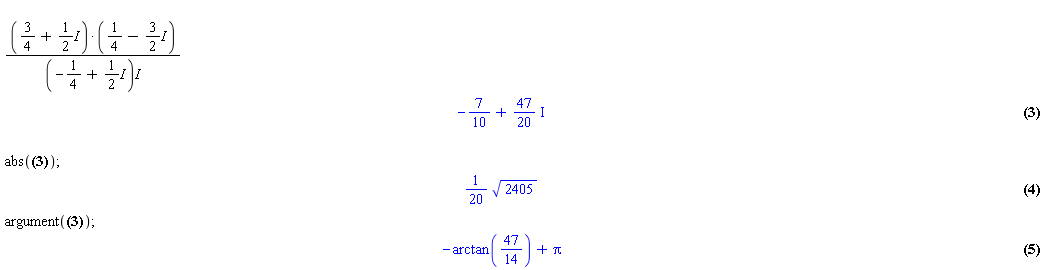
\includegraphics[scale=0.6]{3.png}
\end{center}
\footnote{3-tallet i udregningerne refererer til det komplekse tal som er givet i opgaven 1.3a}Modulus er altså: $\dfrac{1}{20}\sqrt{2405}$ og argumentet er: $-\arctan(\dfrac{47}{14})+\pi$\\
Det komplekse tal kan nu plottes i den komplekse plan ved hjælp af Maple, og ser således ud:
\begin{center}
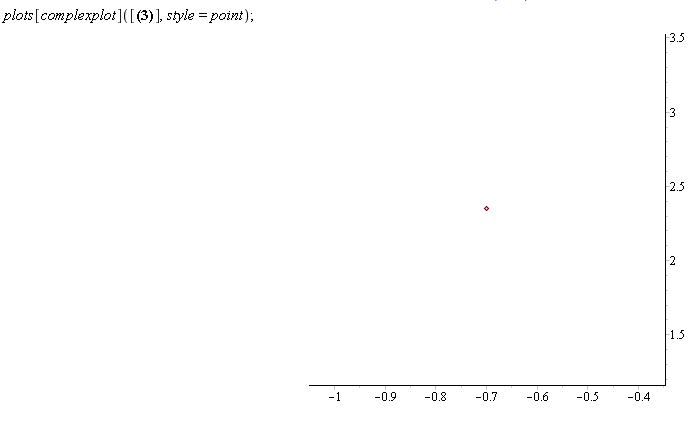
\includegraphics[scale=0.6]{4.png}
\end{center}
Lad nu $z=\dfrac{3}{4}+\dfrac{1}{2}i$. Der skal nu indtegnes følgende punkter i den komplekse plan
$$z^{-8},z^{-7},\ldots, z^{-1},z^{0},z,z^2,\ldots,z^8 $$
og dette gøres hjælp hjælp af følgende Maple kommando:
\begin{center}
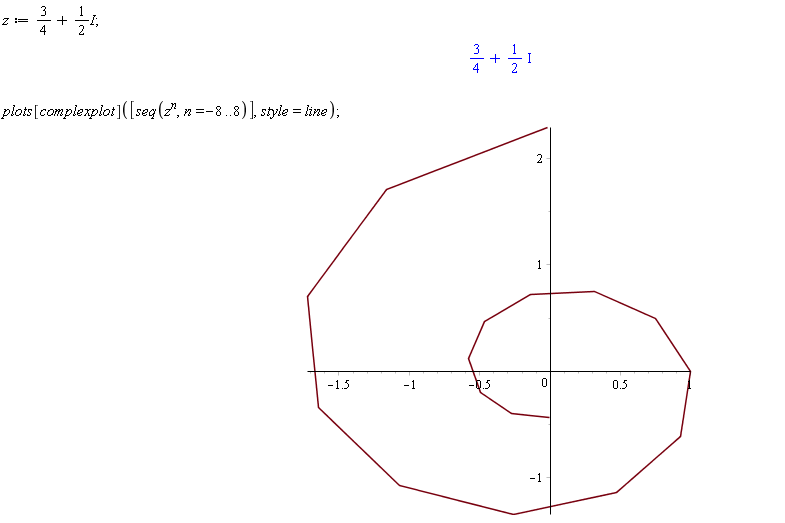
\includegraphics[scale=0.6]{5.png}
\end{center}
Det overstående er en vektorfunktion. Vi observerer at der er reelle tal idet den rammer tallinjen for de reelle tal.\\
Strukturen skyldes, fra TLO teorem 3.2.3, som siger når 2 komplekse tal, med modulus $r_1$ og $r_2$ og argument $\Theta_1$ og $\Theta_2$, ganges sammen vil modulus af tallet være $r_1r_2$ og argumentet vil være $\Theta_1+\Theta_2$. Da det komplekse tal vi kigger på ligger i intervallet $(-1,1)$ for både $a$ og $b$ vil det medføre modulus bliver mindre jo større $n$ bliver og modulus bliver større jo mindre $n$ bliver.\\
Argumentet vil desuden vokse lineært da argumentet til $z^n$ er givet ved $n*\Theta$ hvor $\Theta$ er argumentet til $z$.
\end{document}
